\documentclass[a4paper,11pt]{article}

\usepackage{latexsym}
\usepackage[empty]{fullpage}
\usepackage{titlesec}
\usepackage{marvosym}
\usepackage[usenames,dvipsnames]{color}
\usepackage{verbatim}
\usepackage{enumitem}
\usepackage[hidelinks]{hyperref}
\usepackage{fancyhdr}
\usepackage[english]{babel}
\usepackage{tabularx}
\usepackage{fontawesome5}
\usepackage{multicol}
\usepackage{graphicx}
\usepackage{ragged2e}
\setlength{\multicolsep}{-3.0pt}
\setlength{\columnsep}{-1pt}
\usepackage{iftex}
\ifPDFTeX\input{glyphtounicode}\fi

\pagestyle{fancy}
\fancyhf{}
\fancyfoot{}
\renewcommand{\headrulewidth}{0pt}
\renewcommand{\footrulewidth}{0pt}

\addtolength{\oddsidemargin}{-0.6in}
\addtolength{\evensidemargin}{-0.5in}
\addtolength{\textwidth}{1.19in}
\addtolength{\topmargin}{-.7in}
\addtolength{\textheight}{1.4in}

\urlstyle{same}

\raggedbottom
\raggedright
\setlength{\tabcolsep}{0in}

\titleformat{\section}{
  \vspace{-4pt}\scshape\raggedright\large\bfseries
}{}{0em}{}[\color{black}\titlerule \vspace{-5pt}]

\ifPDFTeX\pdfgentounicode=1\fi

\newcommand{\resumeItem}[1]{
  \item\justifying\small{
    {#1 \vspace{-2pt}}
  }
}

\newcommand{\classesList}[4]{
    \item\small{
        {#1 #2 #3 #4 \vspace{-2pt}}
  }
}

\newcommand{\resumeSubheading}[4]{
  \vspace{-2pt}\item
    \begin{tabular*}{1.0\textwidth}[t]{l@{\extracolsep{\fill}}r}
      \textbf{#1} & \textbf{\small #2} \\
      \textit{\small#3} & \textit{\small #4} \\
    \end{tabular*}\vspace{-7pt}
}

\newcommand{\resumeSubSubheading}[2]{
    \item
    \begin{tabular*}{0.97\textwidth}{l@{\extracolsep{\fill}}r}
      \textit{\small#1} & \textit{\small #2} \\
    \end{tabular*}\vspace{-7pt}
}

\newcommand{\resumeProjectHeading}[2]{
    \item
    \begin{tabular*}{1.001\textwidth}{l@{\extracolsep{\fill}}r}
      \small#1 & \textbf{\small #2}\\
    \end{tabular*}\vspace{-7pt}
}

\newcommand{\hobbyIcon}[1]{\makebox[1.7em][l]{\raisebox{-0.1\height}{\normalsize #1}}}

\newcommand{\resumeSingleHeading}[2]{
  \vspace{-2pt}\item
    \begin{tabular*}{1.0\textwidth}[t]{l@{\extracolsep{\fill}}r}
      \textbf{#1} & \textbf{\small #2} \\
    \end{tabular*}\vspace{-4pt}
}

\newcommand{\resumeSubItem}[1]{\resumeItem{#1}\vspace{-4pt}}

\renewcommand\labelitemi{$\vcenter{\hbox{\tiny$\bullet$}}$}
\renewcommand\labelitemii{$\vcenter{\hbox{\tiny$\bullet$}}$}

\newcommand{\resumeSubHeadingListStart}{\begin{itemize}[leftmargin=0.0in, label={}]}
\newcommand{\resumeSubHeadingListEnd}{\end{itemize}}
\newcommand{\resumeItemListStart}{\begin{itemize}[itemsep=2pt, topsep=3pt, parsep=0pt]}
\newcommand{\resumeItemListEnd}{\end{itemize}\vspace{4pt}}

\begin{document}

\newcommand{\contactIcon}[1]{\makebox[1.7em][l]{\raisebox{-0.15\height}{\Large #1}}}
\begin{minipage}[c]{1.15in}
    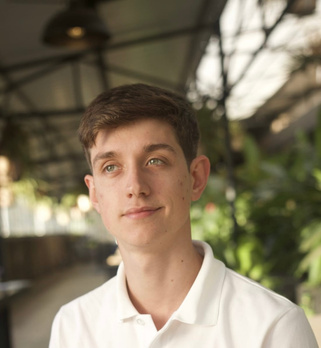
\includegraphics[width=1.15in, height=1.15in, keepaspectratio]{resume_photo.jpg}
\end{minipage}%
\hspace{0.25in}%
\begin{minipage}[c]{\dimexpr\textwidth-1.4in\relax}
    \centering
    {\Huge \scshape Justin Mayer} {\Large \ -- \textit{Software Engineer}} \\[6pt]
    \large
    \begin{tabular}{@{}l@{\hspace{2.5em}}l@{}}
      \contactIcon{\faPhone} +230 5921 3244 &
      \href{mailto:jusmayer@outlook.com}{\contactIcon{\faEnvelope} jusmayer@outlook.com} \\[2pt]
      \href{https://www.linkedin.com/in/jpjmayer/}{\contactIcon{\faLinkedin} jpjmayer} &
      \href{https://github.com/ReyJust}{\contactIcon{\faGithub} ReyJust} \\
    \end{tabular}
\end{minipage}
\vspace{-4pt}

\section{Professional Summary}
{\justifying\small Software Engineer with 4+ years building full-stack web applications, background processing systems and data pipelines with TypeScript and Python. Delivers end to end, from email queues handling thousands of messages daily to a 50\% faster dashboard and stack-wide observability with OpenTelemetry, and gets up to speed quickly in existing codebases. Growing focus on AI: LLM tool-calling chatbots and document AI features, with AI-assisted development as part of the daily workflow.\par}
\small
\vspace{-6pt}

\section{Experience}
  \resumeSubHeadingListStart

    \resumeSingleHeading
      {Career Break \textnormal{-- \textit{Working Holiday, Australia}}}{Feb 2026 -- Dec 2026}

    \resumeSubheading
      {Software Engineer}{Jan 2025 -- Dec 2025}
      {LeadsCloser.ai}{}
      \resumeItemListStart
        \resumeItem{Led frontend refactor of a web application to modern UI frameworks (shadcn/ui), encapsulating legacy modules so the app could be migrated progressively with zero downtime, improving maintainability and UX consistency}
        \resumeItem{Containerized the application with Docker to simplify CI/CD, and handled production deployments, including rolling out Prisma migrations on PostgreSQL and recovering from failed ones}
        \resumeItem{Implemented OpenTelemetry across 3 interconnected systems with a self-hosted Grafana LGTM backend (Prometheus, Tempo, Loki), unifying their logs into single end-to-end traces and adding alerts that sped up debugging and improved uptime}
        \resumeItem{Designed and improved distributed background processing using BullMQ and Redis for thousands of emails daily, including a rate-limiting algorithm to stay within sending caps}
        \resumeItem{Built APIs and LangChain tools for an AI-powered chatbot (Python, FastAPI) with a Vue.js frontend, working across the full conversation cycle from user message to tool calls and response}
        \resumeItem{Optimized backend performance through SQL procedure development, in-database cron jobs, and query tuning, improving dashboard performance by 50\%}
        \resumeItem{Developed scalable web scraping pipelines to extract data from dozens of websites in parallel}
        \resumeItem{Developed Oracle APEX applications, writing SQL procedures and backend logic}
        \resumeItem{Resolved client-reported bugs through a ticketing system, communicating directly with clients from report to fix}
      \resumeItemListEnd

    \resumeSubheading
      {Freelance Software Developer}{2023 -- 2026}
      {BlueBoa Ltd, Catamaran Cruises and others}{Part-time}
      \resumeItemListStart
        \resumeItem{Built around 8 landing-page websites for small businesses, mostly with Elementor and some with custom WordPress themes}
        \resumeItem{Migrated 6 client websites to new hosting, taking over from previous IT providers and handing full ownership back to the owners}
        \resumeItem{Turned provided Figma designs into responsive, production-ready websites}
        \resumeItem{Built multi-threaded Python web scrapers for website with 10,000 pages}
      \resumeItemListEnd

    \resumeSubheading
      {Junior Software Developer}{Apr 2021 -- Dec 2024}
      {Dodobird.ai}{Part-time during studies until Apr 2023}
      \resumeItemListStart
        \resumeItem{Built e-commerce plugins for WordPress, Shopify and nopCommerce, including a WordPress plugin that displays AI product recommendations and embeds a Vue.js chatbot}
        \resumeItem{Implemented full-stack features with Vue.js and Node.js (Express, TypeScript, PostgreSQL), including a queued bulk data import}
        \resumeItem{Built a source-agnostic CRM data ingestion pipeline in Python with Kedro, scheduled with Apache Airflow, processing hundreds of thousands of records}
      \resumeItemListEnd

  \resumeSubHeadingListEnd

\section{Projects}
  \resumeItemListStart
    \resumeItem{\textbf{Praline Recognition:} Tool built to speed up checkout at an Australian café and chocolatier. Identifies pralines from a photo with 93\% accuracy using Azure AI Content Understanding, matching against a text description of each praline, then shows the POS checkout steps to follow}
    \resumeItem{\textbf{Prep:} Nutrition and budget tracking app (in development), with receipt scanning and nutrition-label extraction built on Azure AI Content Understanding}
    \resumeItem{\textbf{\href{https://www.zetpa-mauritius.com}{\underline{Zetpa}}:} Flutter surplus food marketplace for Mauritius (built, not currently operating), letting businesses sell unsold food at a third of the price at the end of the day to reduce food waste; integrated Peach Payments and Google Maps}
    \resumeItem{\textbf{\href{https://osinvoice.vercel.app}{\underline{OsInvoice}}:} Invoicing app for sole traders that generates PDF invoices and drafts the client email automatically; used day to day for real sole-trader invoicing}
    \resumeItem{\textbf{\href{https://github.com/ReyJust/Mauritius_Forex}{\underline{Mauritius Forex}}:} Scraper that collects Mauritian rupee exchange rates automatically every business day and serves them as a free, API-like dataset through GitHub raw content}
  \resumeItemListEnd

\section{Skills}
  \resumeItemListStart
    \resumeItem{\textbf{Programming:} TypeScript, JavaScript, Python, SQL, PHP, C\#}
    \resumeItem{\textbf{Web:} Vue.js, React, Next.js, Node.js, FastAPI, PostgreSQL, Prisma, Redis, BullMQ, WordPress}
    \resumeItem{\textbf{Mobile:} Flutter, React Native, Google Maps, Peach Payments}
    \resumeItem{\textbf{AI:} LangChain, OpenAI and Claude SDKs, Azure AI Foundry, Azure AI Content Understanding}
    \resumeItem{\textbf{Data Processing:} Python, Pandas, Jupyter Notebook, Kedro, Apache Airflow, web scraping}
    \resumeItem{\textbf{Cloud \& DevOps:} AWS, Azure, Docker, CI/CD with GitHub Actions, OpenTelemetry, Grafana}
    \resumeItem{\textbf{Strengths:} versatility, teamwork, proactive adoption of AI tools, quickly navigating and maintaining existing codebases, problem-solving, attention to detail and code quality}
  \resumeItemListEnd

\section{Education}
  \resumeItemListStart
    \item\small{\textbf{GitHub Actions (GH-200)} -- \textit{Microsoft} \hfill Nov 2026}
    \item\small{\textbf{Azure AI Apps and Agents Developer Associate (AI-103)} -- \textit{Microsoft} \hfill Jul 2026}
    \item\small{\textbf{Claude Code and Claude API courses} -- \textit{Anthropic Academy} \hfill Jun 2026}
    \item\small{\textbf{Bachelor of Computer Science, First Class Honours} -- \textit{Middlesex University} \hfill Oct 2020 -- Apr 2023}
  \resumeItemListEnd

\section{Languages}
  \resumeItemListStart
    \resumeItem{French (Native)}
    \resumeItem{English (Proficient)}
    \resumeItem{Mauritian Creole (Fluent)}
  \resumeItemListEnd

\section{Hobbies \& Interests}
  {\centering\small
  \begin{tabular}{@{}l@{\hspace{5em}}l@{}}
    \hobbyIcon{\faRunning} \textbf{Running} &
    \hobbyIcon{\faCampground} \textbf{Scouting:} Assistant Scout Leader \\[2pt]
    \hobbyIcon{\faUtensils} \textbf{Cooking \& Baking} &
    \hobbyIcon{\faHeartbeat} \textbf{Health, Fitness \& Nutrition} \\
  \end{tabular}\par}

\end{document}
